\section{Trigger requirements}
Events analyzed in this note are recorded using Beam Scintillation
Counter (BSC) system at CMS. BSC system provides a set of ``technical'' triggers which
could be used to identify collision candidates. Events collected by this
triggers are found in the Minimum Bias dataset. 

For this analysis we select collision candidates using the following
Level-1 technical trigger (TT) selections:

\begin{itemize}
\item At least one of the BSC MinBias TT was fired:
  L1Tech\_BSC\_minBias\_threshold1 (TT bit 40) or
  L1Tech\_BSC\_minBias\_threshold2 (TT bit 41). These triggers fire when
  there is a coincident activity in the forward and backward BSC
  detectors, indicating a collision candidate.
\item None of the BSC beam halo triggers fired:
  L1Tech\_BSC\_halo\_beam2\_inner (TT bit 36),
  L1Tech\_BSC\_halo\_beam2\_outer (TT bit 37),
  L1Tech\_BSC\_halo\_beam1\_inner (TT bit 38),
  L1Tech\_BSC\_halo\_beam1\_outer (TT bit 39). These triggers fire when
  the hits in the forward and backward BSC detectors are inconsistent in
  timing with originating from the collision.
\end{itemize}

In addition to the Level-1 TT bit selections, we also require that the
HLT trigger bit ``HLT\_PhysicsDeclared' bit is set, which indicates that
the high voltages of the CMS pixel detector and the tracker are turned
on.

In this analysis we process the data collected during the LHC
commissioning phase during the December 2009 data-taking at CMS. During
this period the majority of collisions were at $\sqrt{s}=900$~GeV, and a
smaller dataset was collected with $\sqrt{s}=2.36$~TeV.

\section{Data Samples}

Events analyzed in this study are selected from the Minimum Bias
dataset, which was reconstructed on Dec 14, 2009 using
CMSSW\_3\_3\_5\_patch4. We used the data sample which has the the
trigger selections discussed in the previous section are already
applied:
\begin{itemize}
\item
  /MinimumBias/BeamCommissioning09-BSCNOBEAMHALO-Dec14thSkim\_v1/RAW-RECO
\end{itemize}
Additionally, we require that L1 TT bit 0 was also fired, which
indicates consistent timing with LHC bunch crossing.

We require that the events considered in this analysis were collected
during the runs with no ``known'' problems in the
calorimeters. Therefore, the run selection for this analysis is based on
the good run list from the JetMET DQM group. This list is also compared
to the ECAL and HCAL DPG groups' list of known bad runs. 

For the $\sqrt{s}=900$~GeV data-taking period the following runs were
identified to have no known problems and are studied in this analysis:
122314, 123575, 123586, 123587, 123591, 123592, 123596, 123600, 123603,
123606, 123608, 123740, 123801, 123815, 123818, 123893, 123906, 123908,
123909, 123910, 124017, 124019, 124020, 124022, 124023, 124024, 124025,
124026, 124027, 124029, 124030, 124108, 124115.

For the $\sqrt{s}=2.36$~TeV data-taking period only two runs were
selected: 124119 and 124120.

\subsection{Monte Carlo simulation}

The collision data events considered in this analysis are compared with
{\sc pythia} simulations of Minimum Bias collisions which are processed
with {\sc GEANT-4} simulation of the CMS detector. The Monte Carlo
simulation is then reconstructed using CMSSW\_3\_3\_5\_patch2. The data
sample corresponding to this sample can be found at:
\begin{itemize}
\item /MinBias/Summer09-STARTUP3X\_V8I\_900GeV-v2/GEN-SIM-RECO
\end{itemize}
For the comparisons of data with simulation we require that
simulated events pass the BSC Minimum Bias trigger selections (TT bits
40 and 41). Additionally, any further selections described in the next
section are applied to both data and simulation.

\section{Event Selection}

\subsection{Vertex selection}

In order to further constrain the event selection to identify the
collision events, several studies have considered a selection based on
the reconstructed primary vertex properties, such as $Z$ position or
number of tracks attached to the vertex. The comparison of the vertex
$Z$ distribution in data compared to simulation is shown on
Fig.\ref{fig:vertex_selection_1}. Events shown in
Fig.\ref{fig:vertex_selection_1}  are required to have at least 2 tracks
attached to the primary vertex. As can be seen from this comparison,
the simulation does not agree well with the observed distribution of
this variable. Therefore, we choose not to make any selection on this variable.

\begin{2figures}{hbtp}
  \resizebox{8cm}{!}{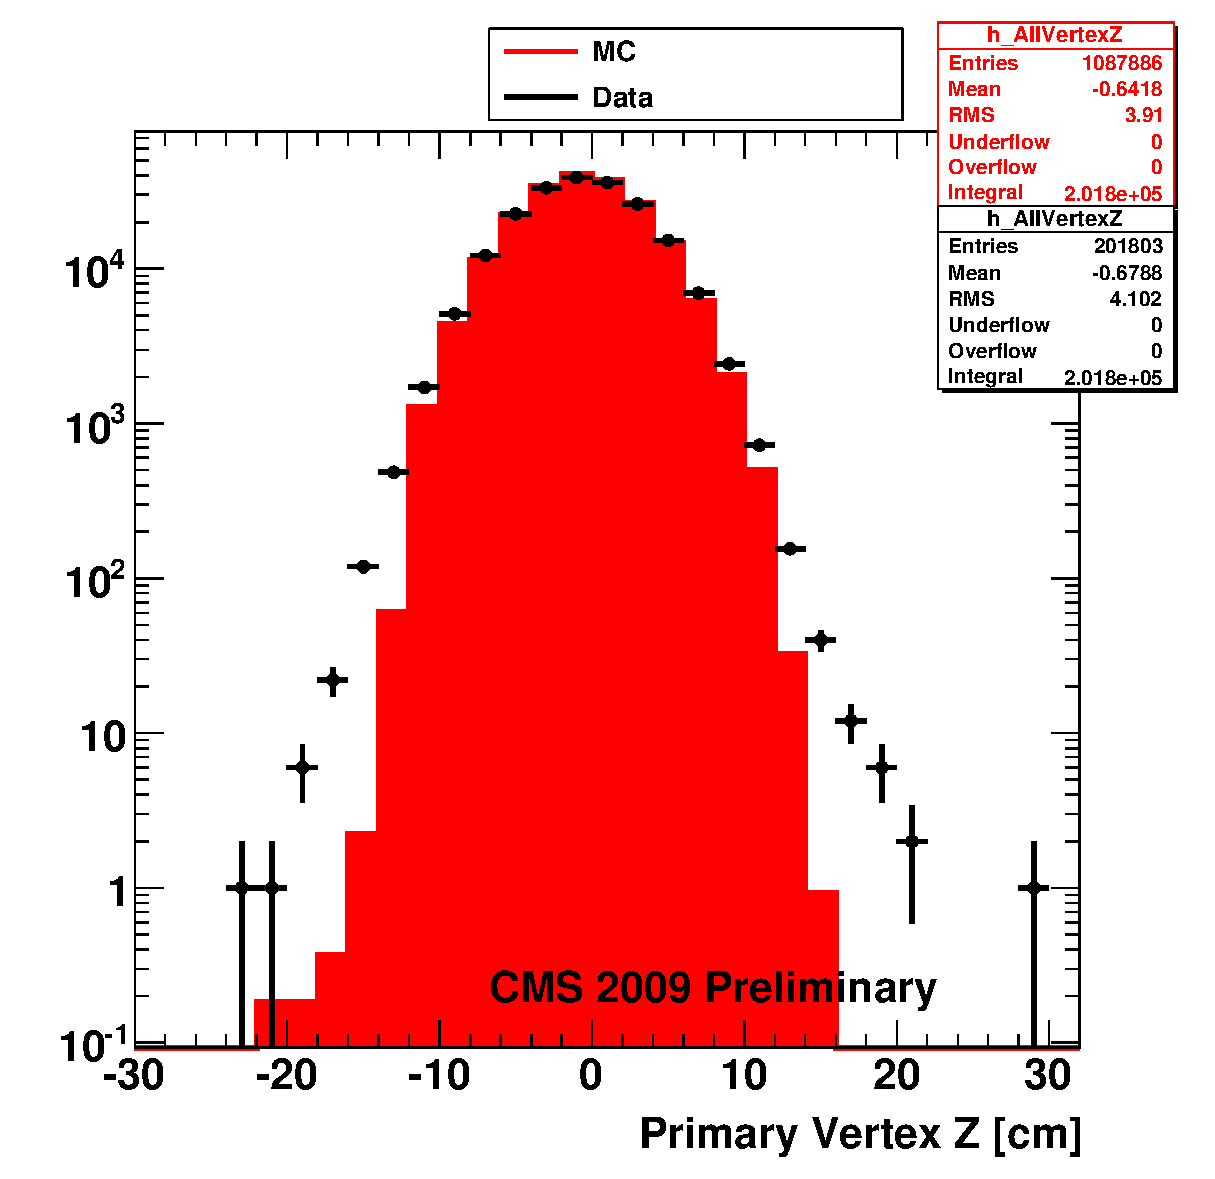
\includegraphics{plots_EventSelection/h_AllVertexZ_log.eps}} &
  \resizebox{8cm}{!}{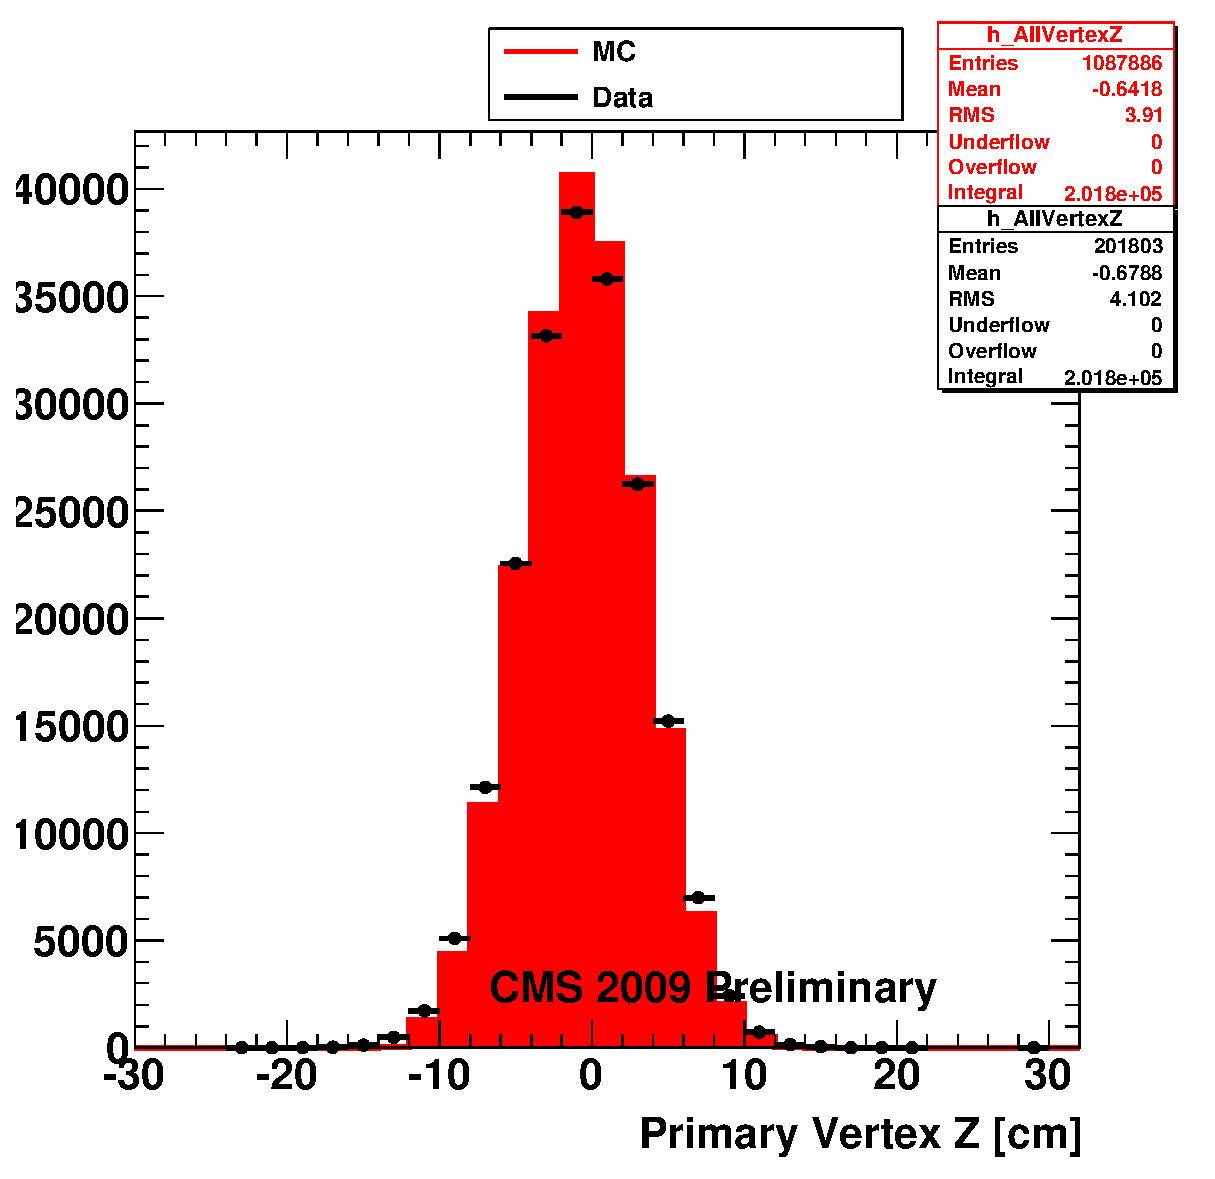
\includegraphics{plots_EventSelection/h_AllVertexZ_linear.eps}} \\
 \label{fig:vertex_selection_1}
\caption{Comparison of the distribution of the event primary vertex $Z$
  position between data and Monte Carlo simulation. Distributions for
  events that have at least two tracks attached to the vertex are shown.}
\end{2figures}

\subsection{Removal of scraping events}

During the LHC commissioning phase of data-taking it was observed that
in some bunch crossings there was a anomalously large occupancy in the
pixel detector, which resulted in a large number of reconstructed fake
tracks. These events were identified as being the result of beam
particles traversing the pixel detector longitudinally. We reject this
type of events by requiring that the fraction of high-purity tracks in
all events with more than 10 tracks is greater than 20\%.

\subsection{HCAL anomalous noise}
Commissioning studies of the CMS hadronic calorimeter performed 
during past Test Beam, Cosmic and Beam runs have identified 
sporadic noise events CMS PAPER CFT-09-019.
Intermittent anomalous signals observed so far can be grouped in two categories:
\begin{itemize}
\item{HB/HE atypical signals} Ion Feedback (typically 1-2 channels in one HPD are affected), 
HPD Noise (typically all 18 channels in one HPD are affected), RBX Noise(coherent noise affecting up to 
72 channels in one Readout Box unit);
\item{HF atypical signals} PMT window hits (Occasionally an energetic charged particle directly impinges 
upon the window of an HF PMT rather than striking a HF quartz. This results in an abnormally large 
apparent energy signal for a signal channel within the HF). 
\end{itemize}

The presence of such rare atypical signals was also confirmed in recent 2009 collision data, 
resulting in large $\etmiss$ in the event. 

Preliminary studies performed on a data sample of Mininum Bias events at $\sqrt{s}=900$~GeV 
seems to indicate that HF PMT window hits are significantly more frequent in the tail of MET
then HB/HE related noise events (for $\etmiss>14$~GeV, about 90\% of noise events attributed 
to HCAL is identified as coming from HF; see this talk for more details in 
``http://indico.cern.ch/getFile.py/access?contribId=8\&resId=6\&materialId=slides\&confId=76047'').
This can be explained considering that HF PMT window hits are beam related 
(at this stage probably beam halo muons hitting the PMT window), 
while HB/HE noise events (HPD and RBX noise) are independent from the beam activity; 
therefore the probability of overlap of an HB/HE noise event with a collision event is small.
Studies are ongoing to understand if the rate of HB/HE noise events is consistent with what 
previously observed during CRAFT09.

The list below is an attempt to summarize the 
contributions provided by different people on the identification and rejection of such atypical noise events. 

\begin{itemize}

\item{\bf HCAL studies on HBE/HE noise events} A set of algorithms have been developed by the HCAL group to 
identify and address these types of problems in the data. The methods have been tested on cosmic muon data, 
dedicated calorimeter noise data, and single beam data collected at CMS in 2008, 
as described in CMS PAPER CFT-09-019. A ``HcalNoiseSummary'' object 
is also implemented in CMSSW and it contains basic information useful to identify HB/HE noise events.
More information can be found at 
the CMS Twiki page ``HcalNoiseInfoLibrary''.
Information on HF noise events are not currently stored in the ``HcalNoiseSummary'' object.
The ``HcalNoiseSummary'' object information is not used in the current version of this note
to reject HB/HE noise events.

\item{\bf HCAL studies on HF PMT window hits} PMT windows hits within the HF are tagged by comparing 
the energies reconstructed from long and short fibers with the same ($\eta$,$\phi$) values. 
Given a pair of adjacent long and short 
fibers, with energies $E^L$, $E^S$, respectively, the fiber channels are flagged as noisy if 
(a) the maximum transverse energy $E_T^{max}$ reported by the two channels is at least 5~GeV, and (b) 
if the energy ratio R, defined as:
%
\begin{equation}
R = \frac{E^L - E^S}{E^L + E^S}
\end{equation}
%
is, in module, greater than 0.995. In this study, if at least one HF fiber channel 
is flagged by this algorithm, the event is rejected from the analysis. 
Figure~\ref{fig:hf_noise_longshortFiber} shows the scatter distributions of $E_T^L$($E_T^S$) vs $R$, 
for both data and MC, after applying the full event selection except the HF filter itself.
The HF noise events can be identified by large $E_T^L$($E_T^S$) values and $R$ values close to 1 or -1.
\\
\\
%
\begin{figure}[h!]
 \centering
 \begin{tabular}{ll}
  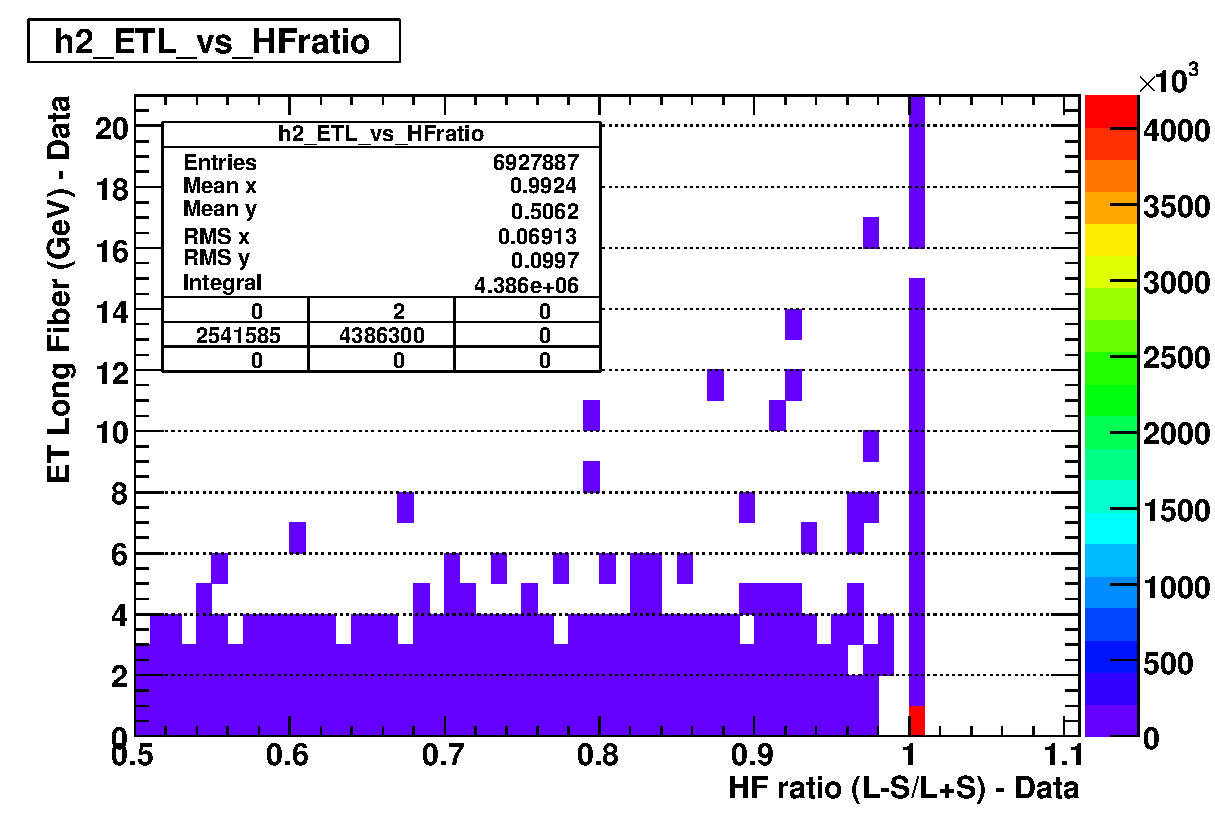
\includegraphics[width=0.5\textwidth]{plots_hcalnoise/hf_longfiberET_vs_ratio_DATA.eps} &
  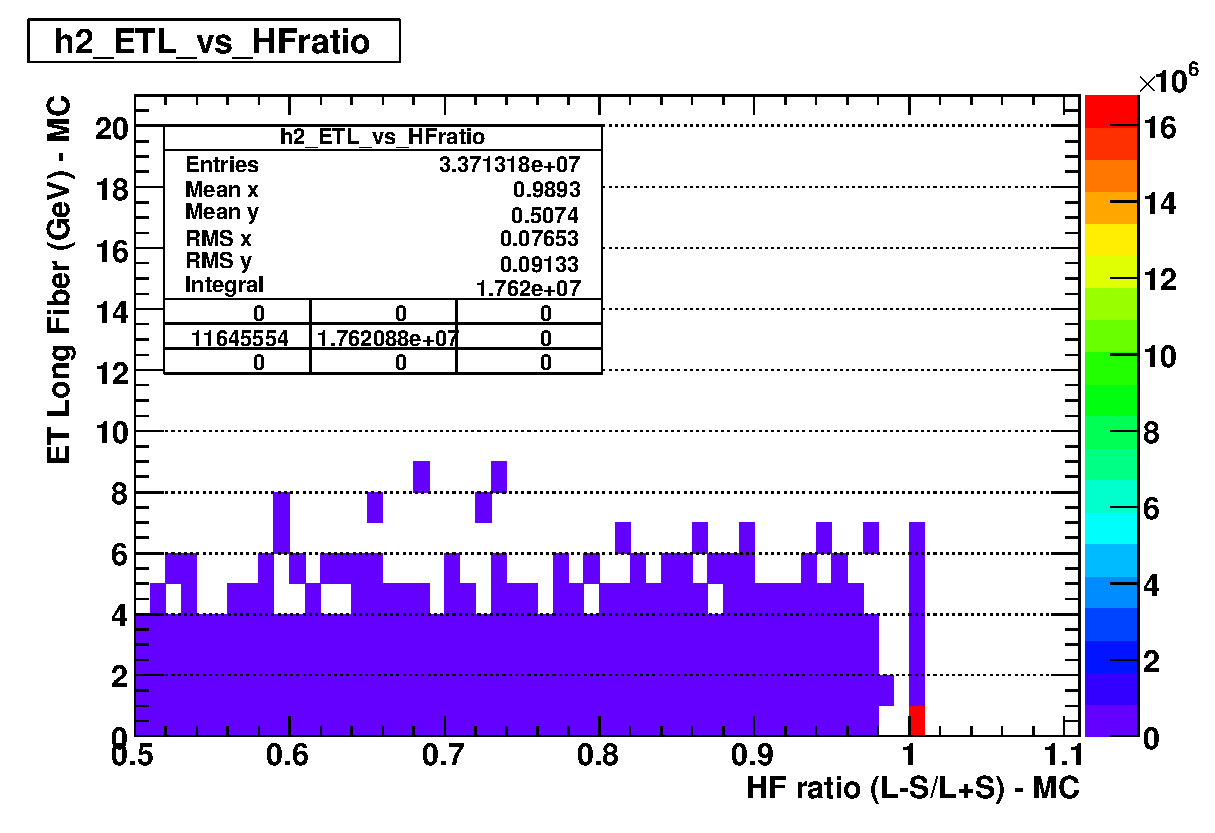
\includegraphics[width=0.5\textwidth]{plots_hcalnoise/hf_longfiberET_vs_ratio_MC.eps} \\
  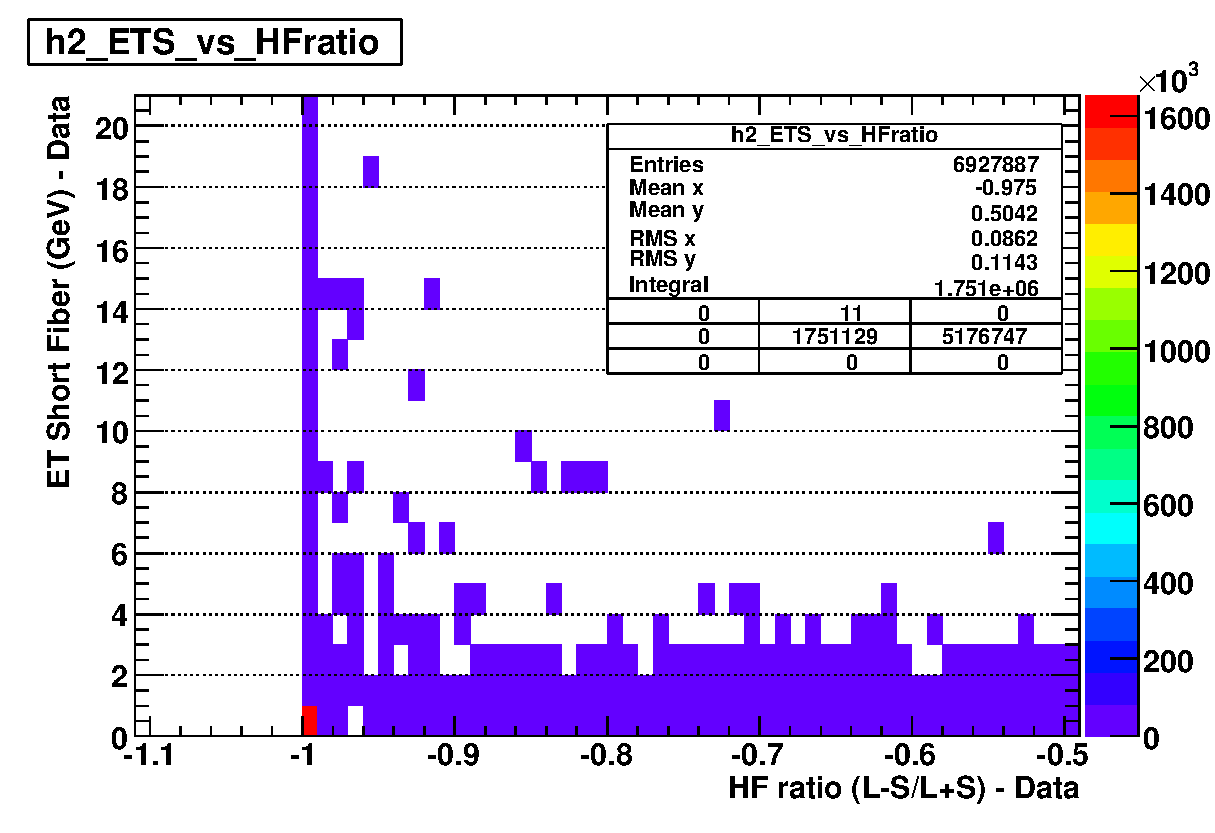
\includegraphics[width=0.5\textwidth]{plots_hcalnoise/hf_shortfiberET_vs_ratio_DATA.eps} &
  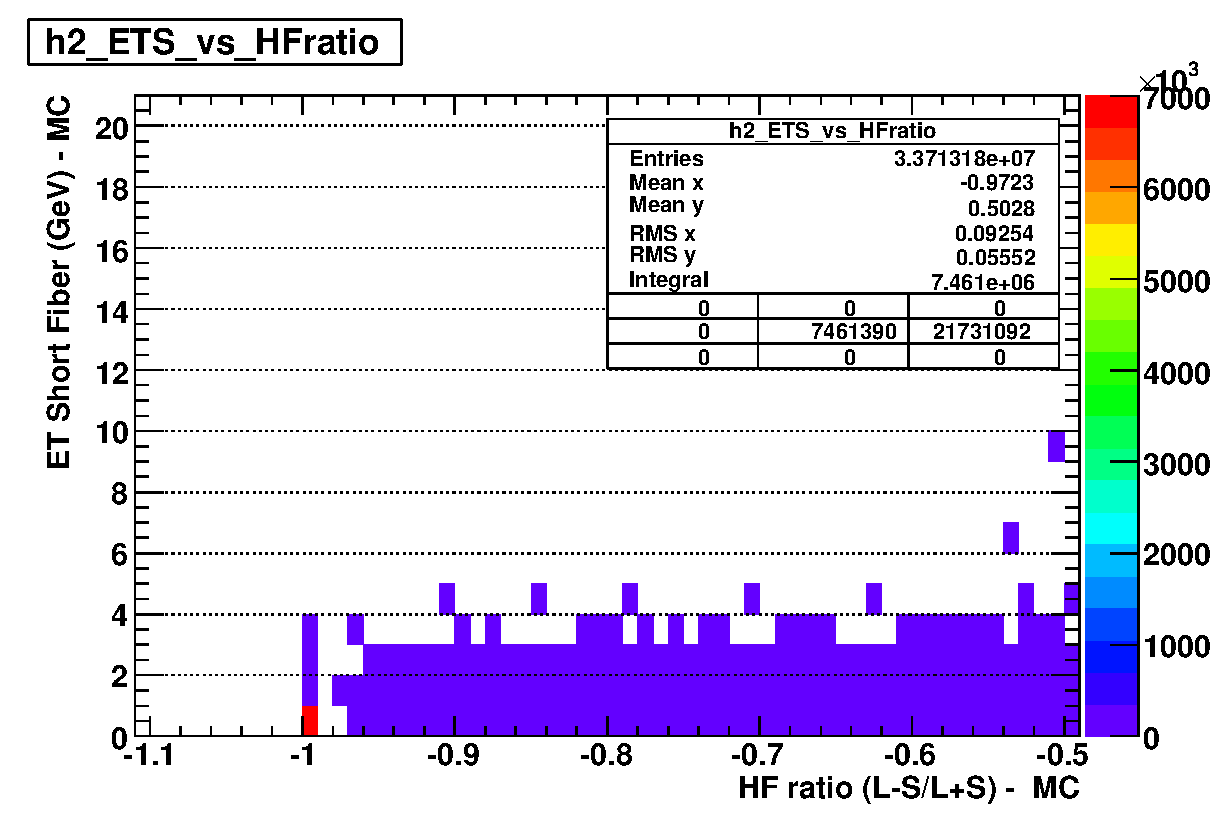
\includegraphics[width=0.5\textwidth]{plots_hcalnoise/hf_shortfiberET_vs_ratio_MC.eps} \\
 \end{tabular}
\caption{\small (Top) Scatter distribution of transverse energy in the long fibers versus $R$ for both data (Left) and MC (Right), 
and (Bottom) distribution of transverse energy in the short fibers versus $R$ for both data (Left) and MC (Right), 
after applying the full event selection except the HF filter itself. 
Plots are filled for each HF tower if either $E_L>1.2$~GeV or $E_S>1.8$~GeV. 
The x axis range is chosen in order to highlight the region where noise events appear. \label{fig:hf_noise_longshortFiber}}
\end{figure}
%

\item{\bf HCAL noise cleaning from PFMET group}
need to be added.

\end{itemize}

\subsection{ECAL anomalous noise}

A set of events with unphysical characteristics in ECAL calorimeter was
observed during the initial analysis of the $\sqrt{s}=900$~GeV data
collected at CMS. These events contain a single, isolated ECAL crystal
with energy deposit (``spike'' crystals), and the crystals were observed
to be uniformly distributed across the ECAL. The
study to efficiently identify the source of this type of events and
efficiently remove them is still ongoing, and here we summarize the set
of selections proposed by different studies. It was observed that this
noise is present both in crossing with and without beam, but there are
indications that the rate is larger in the filled crossings.

One of the first algorithms to reject the spike ECAL events was proposed
by the TcMET group. The ratio of the energy deposited in the spike
crystal ($S1$) to the energy measured in a 3x3 block of crystals ($S9$)
around it is expected to be very small, provided the occupancy in the
ECAL is low. Therefore, a selection of events based on the ratio $S1/S9$
is considered. It has been shown the distribution of $S1/S9$ in data has
a large spike at $1$, which is inconsistent with energy deposition due
to a real photon or electron. It was proposed to identify spike events
by requiring that an ECAL crystal has $E_T>5$~GeV and
$|S1/S9-1|<0.01$. It was observed that by correcting the measured raw
$\etmiss$ with the energy of the spike crystal one can remove
$\sim~30\%$ of the tail in $\etmiss$ distribution.

A different study looked at additional variables associated with spike
events. The variables defined in this study are:
\begin{itemize}
\item NCRY805: Number of crystals with $E>0.08$~GeV in a 5x5 block around the
  spike crystal (in addition to the spike crystal)
\item Rook Fraction: Fraction of energy of the spike crystal that is measured in
  the most energetic neighboring crystal which shares an edge with the spike. This
  fraction is set to $0$ if the energy of the most energetic neighboring
  crystal is below $80$~MeV (80 MeV is $2\sigma$ above noise level in an
  ECAL crystal).
\end{itemize}

The distributions of Rook Fraction (FRook) in data and simulation for
900 and 2360 GeV are shown in Fig.\ref{fig:ecal_noise_1},
\ref{fig:ecal_noise_2} respectively. The ``hybridSuperClusters''
algorithm was used to reconstruct the ECAL clusters. A distinct set of events can
be observed at FRook values below 0.01 across the $E_T$ spectrum of
spike crystal. This feature is not observed in the Monte Carlo
simulation. Figure~\ref{fig:ecal_noise_3} shows the comparison of the
Rook Fraction in data with simulation. For the events considered in this
analysis we chose to identify spike events by requiring that an ECAL
crystal has $E_T>3GeV$ and FRook$<0.01$.

\begin{2figures}{hbtp}
  \resizebox{8cm}{!}{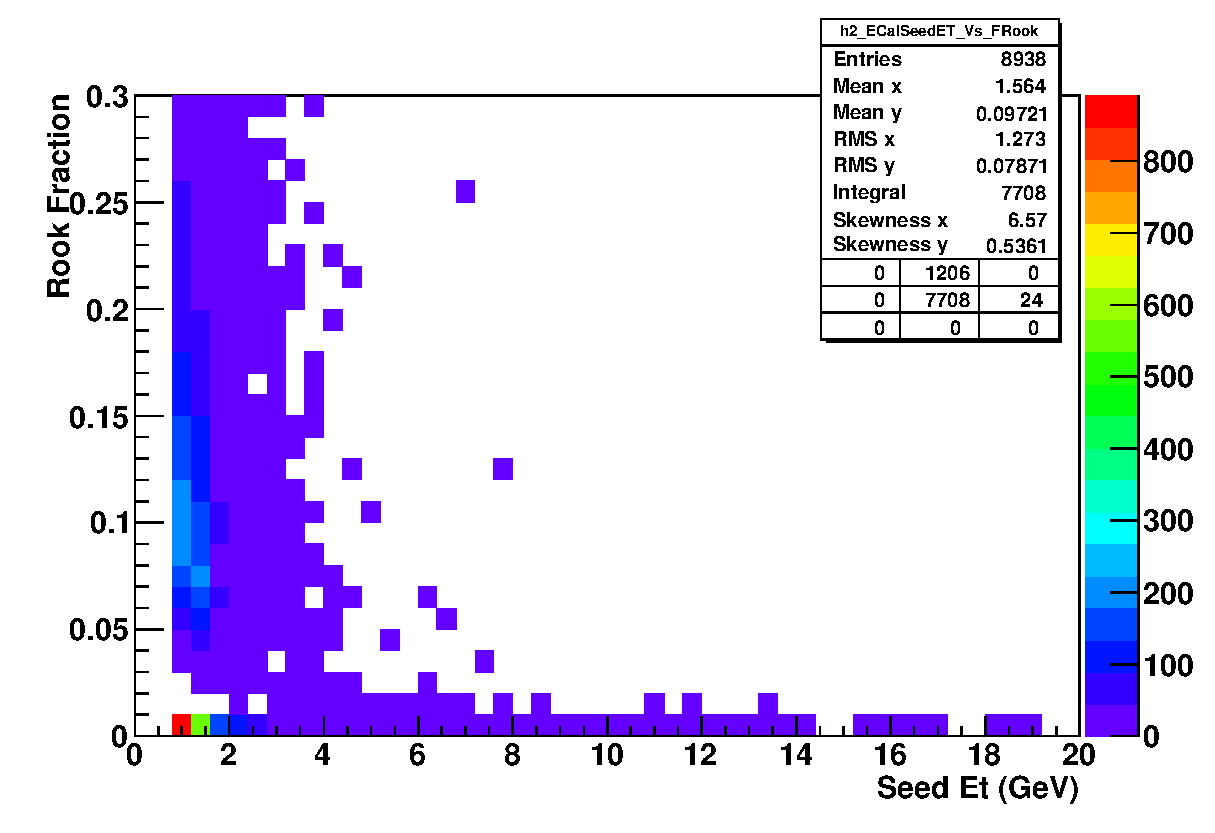
\includegraphics{plots_ecalnoise/SeedET_Frook_DATA900GeV.eps}} &
  \resizebox{8cm}{!}{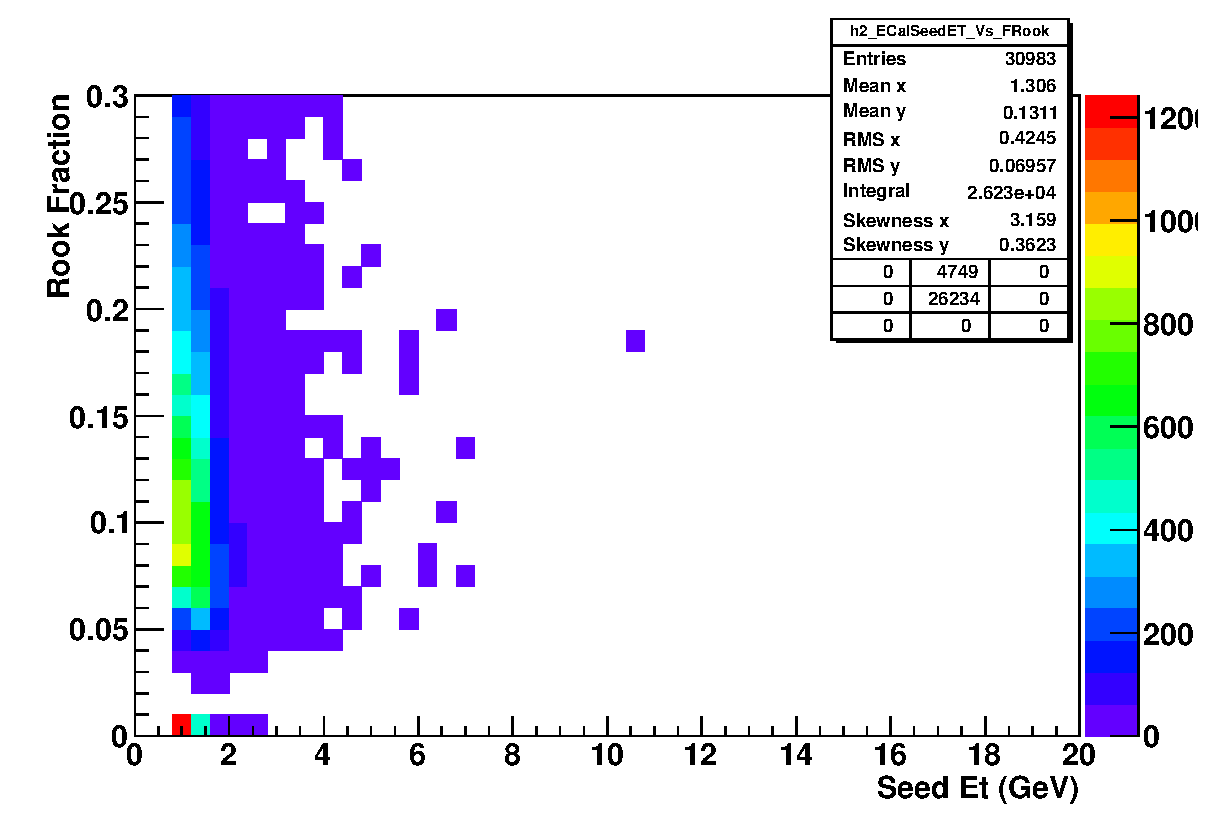
\includegraphics{plots_ecalnoise/SeedET_Frook_MC900GeV.eps}} \\
\caption{Distributions of the Rook Fraction in 900 GeV data and Monte Carlo
  simulation for barrel ECAL. Distributions are shown for events that pass all
  selections described in previous sections.}
\label{fig:ecal_noise_1}
\end{2figures}

\begin{2figures}{hbtp}
  \resizebox{8cm}{!}{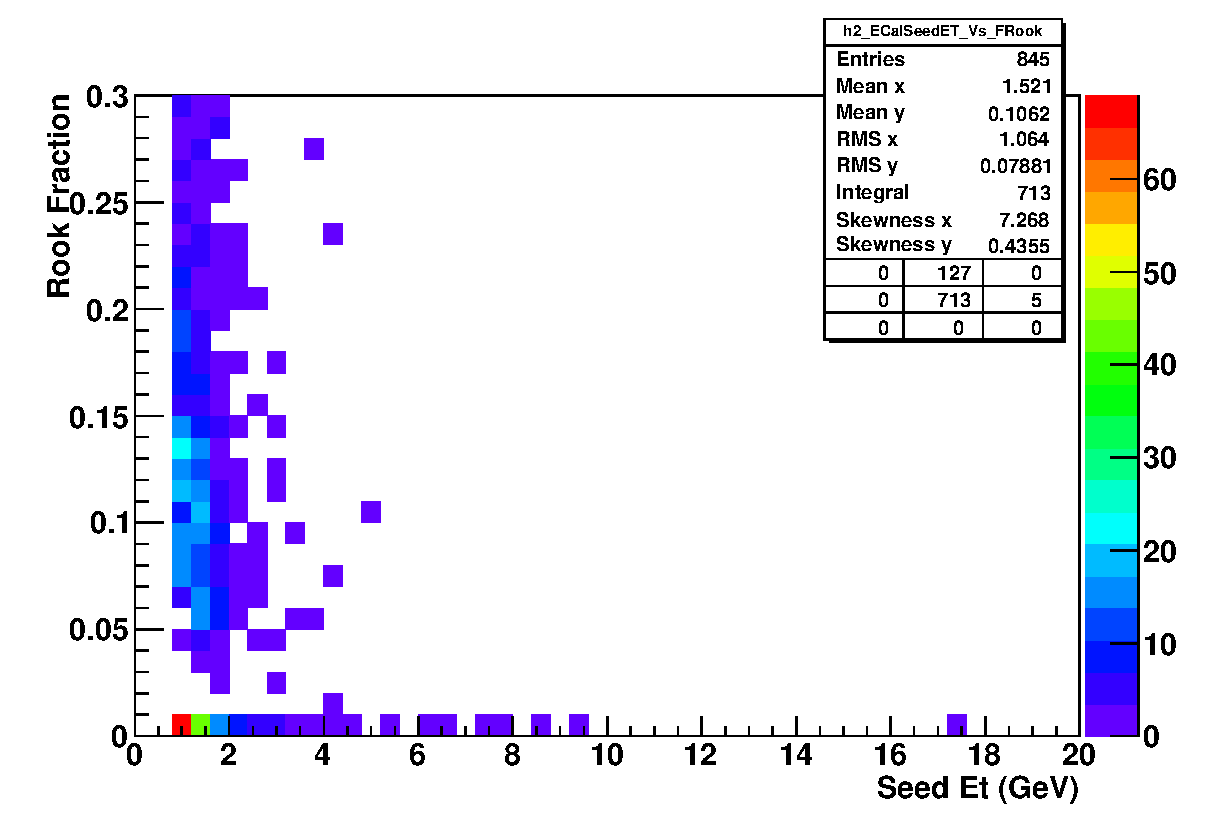
\includegraphics{plots_ecalnoise/SeedET_Frook_DATA2360GeV.eps}} &
  \resizebox{8cm}{!}{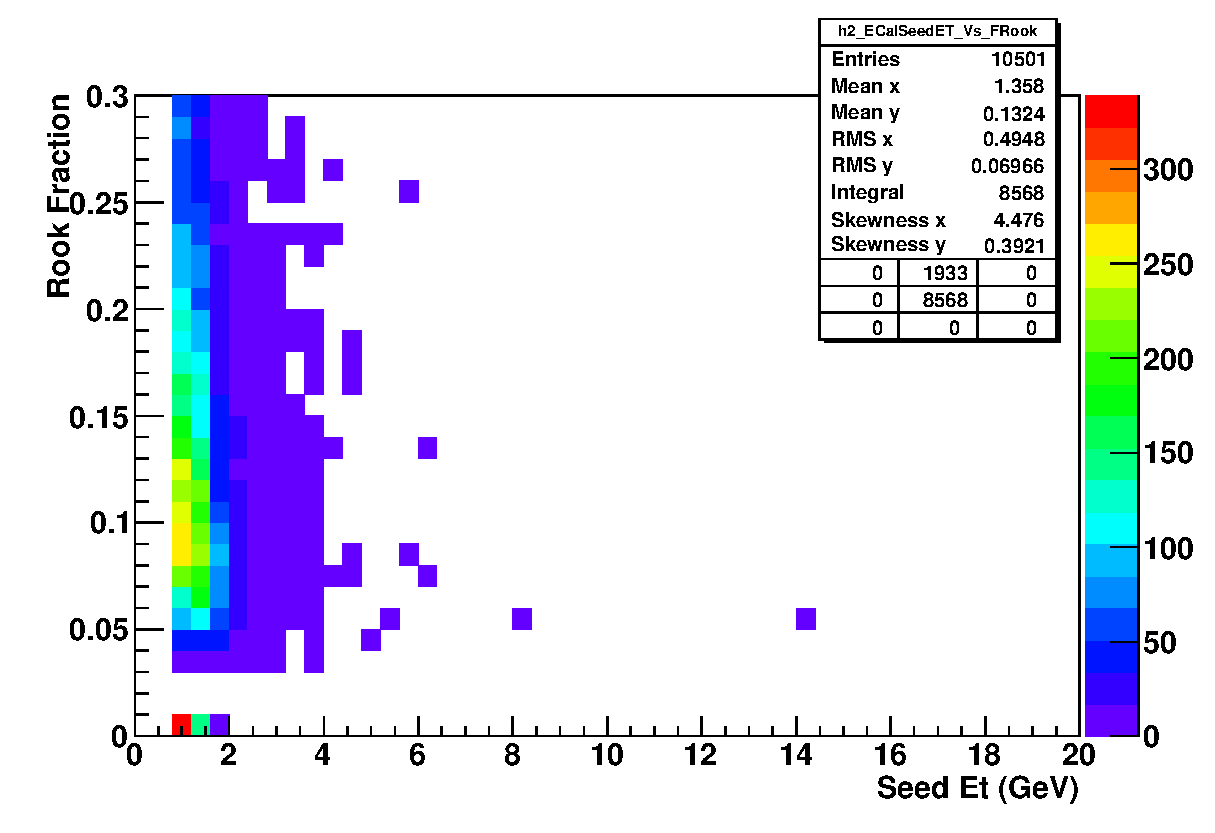
\includegraphics{plots_ecalnoise/SeedET_Frook_MC2360GeV.eps}} \\
\caption{Distributions of the Rook Fraction in 2360 GeV data and Monte Carlo
  simulation for barrel ECAL. Distributions are shown for events that pass all
  selections described in previous sections.}
\label{fig:ecal_noise_2}
\end{2figures}

\begin{2figures}{hbtp}
 \resizebox{8cm}{!}{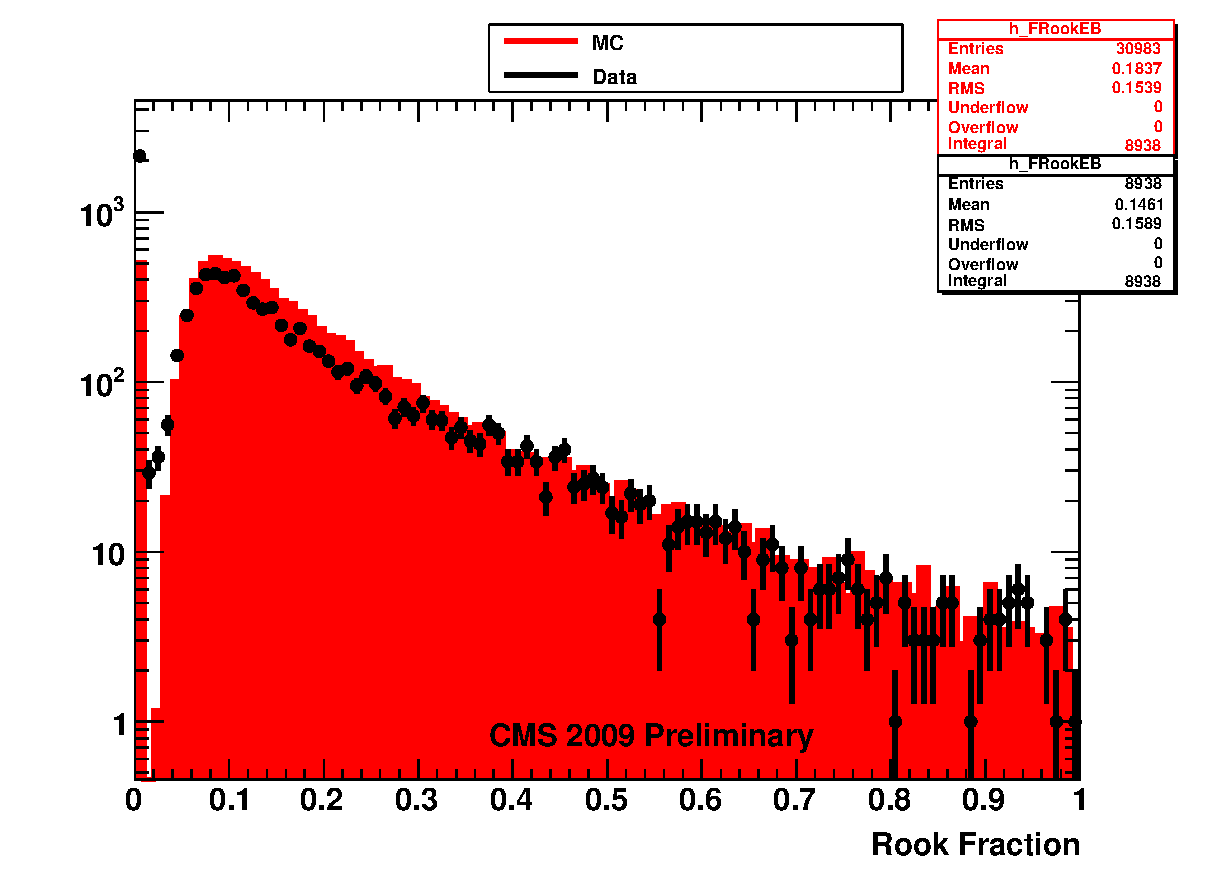
\includegraphics{plots_ecalnoise/Frook_900GeV.eps}}&
  \resizebox{8cm}{!}{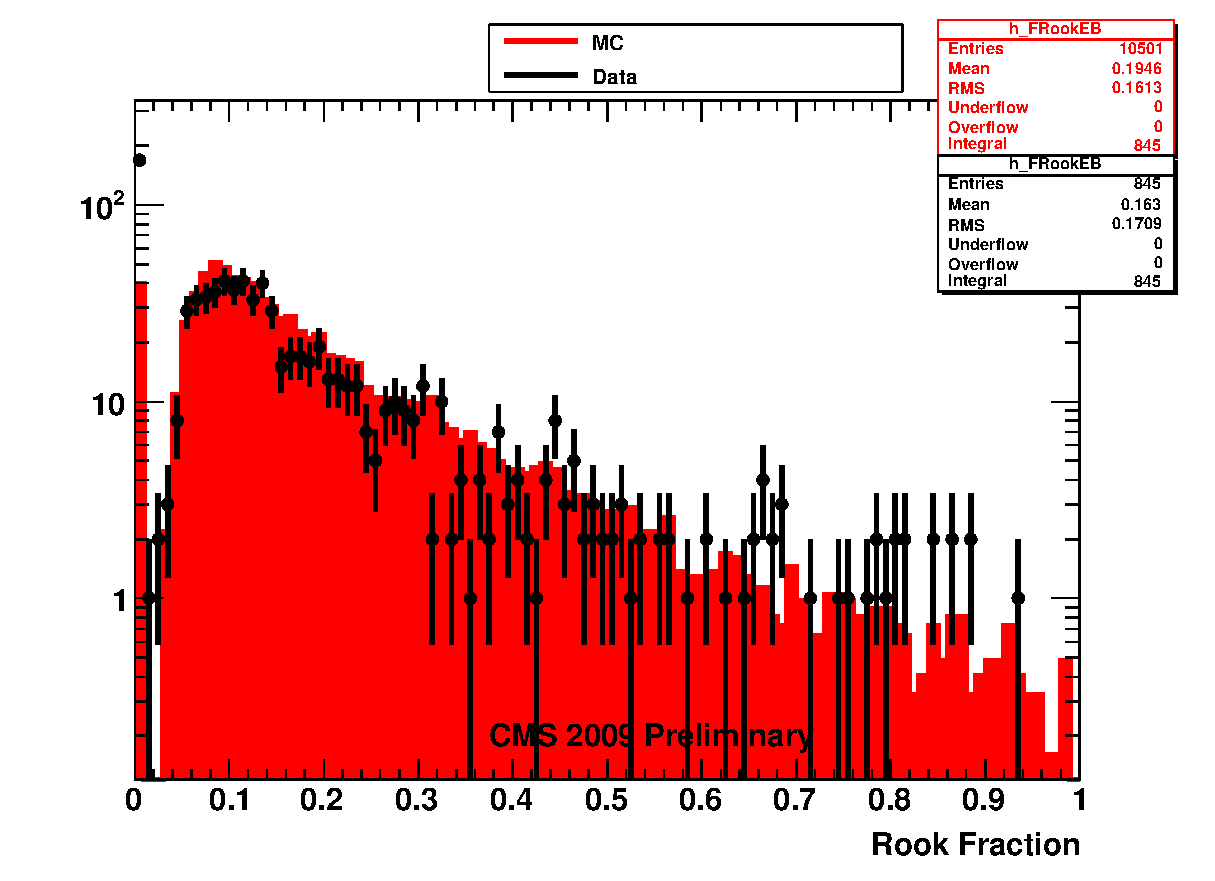
\includegraphics{plots_ecalnoise/Frook_2360GeV.eps}}\\
  \caption{Comparison of the Rook Fraction in 900 and 2360 GeV data and Monte Carlo
  simulation for barrel ECAL. Distributions are shown for events that pass all
  selections described in previous sections.}
\label{fig:ecal_noise_3}
\end{2figures}

Tables~\ref{tab:selectionefficiency_1},\ref{tab:selectionefficiency_2}
summarize the number of events after each set of event selection
criteria defined above, as well as their efficiencies in data and
simulation. Both 900 ans 2360 GeV data samples are considered in these tables.

\begin{table}[!ht]
  \begin{center}
    \begin{tabular}{|c|c|c|c|}
      \hline
      Selection      & Number of Events  & Relative Efficiency   &
      Absolute Efficiency\\
      \hline\hline
      Trigger                            & 303277 (13578) & 1.0 (1.0)&1.0 (1.0) \\ 
      Good Run List                 & 224638 (13578) & 0.74 (1.0) & 0.74(1.0)  \\
      Technical Trigger Bit 0    & 196792 (11069) & 0.88 (0.82) & 0.65 (0.82)\\
      Scraping Events Removal& 195919 (11035) & 0.99 (0.99) & 0.65 (0.81) \\
      HF PMT hits Removal      & 195585 (11007) & 0.99 (0.99) & 0.64 (0.81)\\
      ECAL spikes Removal     & 195301 (10983) & 0.99 (0.99) & 0.64 (0.81) \\ \hline
  \end{tabular}
    \caption{Number of events in the 900~GeV (2360~GeV) data sample and
      the efficiencies of the various event selections applied.}
    \label{tab:selectionefficiency_1}
  \end{center}
\end{table}

\begin{table}[!ht]
  \begin{center}
    \begin{tabular}{|c|c|c|c|}
      \hline
      Selection      & Number of Events  & Relative Efficiency   &
      Absolute Efficiency\\
      \hline\hline
      Good Run List                 & 1442065 (285710) & 1.0 (1.0) & 1.0 (1.0)  \\
      Trigger Selection             & 981765 (142192) & 0.68 (0.50)& 0.68 (0.50) \\ 
      Technical Trigger Bit 0    & 981765 (142192) & 0.68 (0.50) & 0.68 (0.50)\\
      Scraping Events Removal& 981763 (142190) & 0.99 (0.99) & 0.68 (0.50) \\
      HF PMT hits Removal      & 981757 (142185) & 0.99 (0.99) & 0.68 (0.50)\\
      ECAL spikes Removal     & 981757 (142185) & 0.99 (0.99) & 0.68 (0.50) \\ \hline
    \end{tabular}
    \caption{Number of events in the 900~GeV (2360~GeV) Minimum Bias
      Monte Carlo samples and the efficiencies of the various event
      selections applied.}
    \label{tab:{tab:selectionefficiency_2}}
  \end{center}
\end{table}

\subsection{Removal of Cosmic and BeamHalo Events}
to be added.

\subsection{Effect of noise removal}
Here we put the $\etmiss$ distribution with base selection, for the moment just 
after HCAL/ECAL noise removal.

\clearpage
